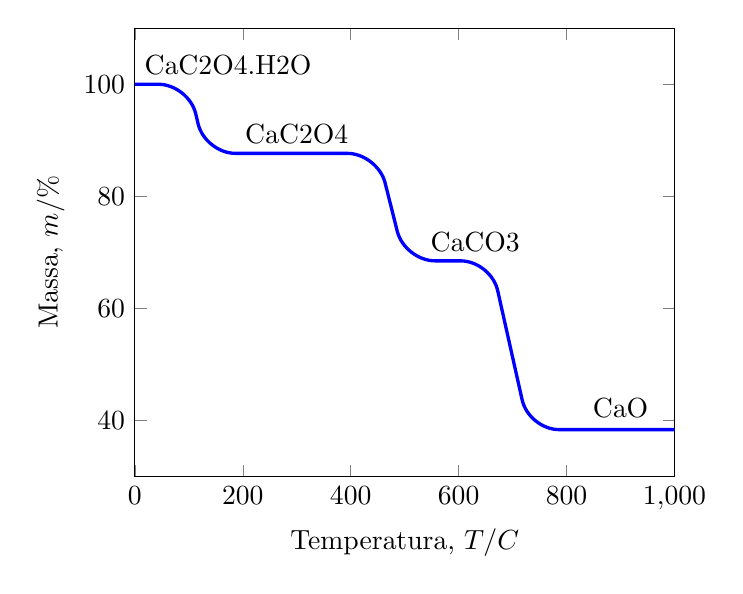
\begin{tikzpicture}
    \begin{axis}
        [
            grid = none,
            ylabel = {Massa, $m/\%$},
            xlabel = {Temperatura, $T/\unit{\degree C}$},
            xmin = 0,  xmax = 1000,
            ymin = 30, ymax = 110,
        ]
    \draw [draw=blue, very thick, rounded corners=1.1em]
        (axis cs:    0, 100.00) --
        (axis cs:  100, 100.00) --
        (axis cs:  130,  87.67) -- 
        (axis cs:  450,  87.67) -- 
        (axis cs:  500,  68.49) -- 
        (axis cs:  660,  68.49) --
        (axis cs:  730,  38.37) --
        (axis cs: 1000,  38.37);

    \node [anchor = south west] at (axis cs:0, 100) 
        { \ce{CaC2O4.H2O} };

    \node [anchor = south] at (axis cs:300, 87.67) 
        { \ce{CaC2O4} };

    \node [anchor = south west] at (axis cs:530, 68.49) 
        { \ce{CaCO3} };

    \node [anchor = south] at (axis cs:900, 38.73) 
        { \ce{CaO} };
    \end{axis}
\end{tikzpicture}

